\begin{frame}{RNN}
    
    \begin{figure}
        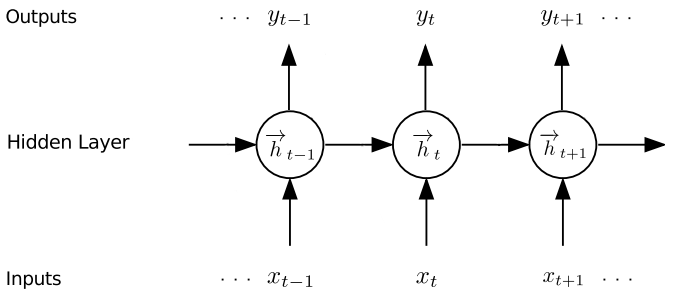
\includegraphics[height=.75\textheight,width=\textwidth,keepaspectratio]{images/arch_rnn}
        \caption{RNN classique {\scriptsize\it -- Source : \cite{Graves13b}}}
    \end{figure}
    
\end{frame}

\begin{frame}{RNN bidirectionnel}
    
    \begin{figure}
        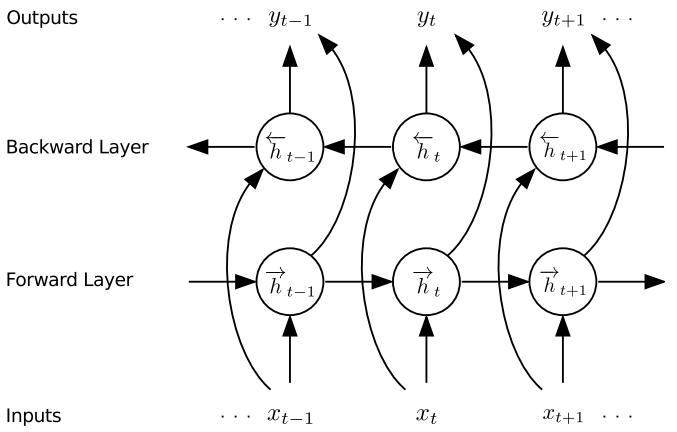
\includegraphics[height=.75\textheight,width=\textwidth,keepaspectratio]{images/arch_brnn}
        \caption{RNN bidirectionnel {\scriptsize\it -- Source : \cite{Graves13b}}}
    \end{figure}
    
\end{frame}

\begin{frame}{RNN bidirectionnel profond}
    
    \begin{figure}
        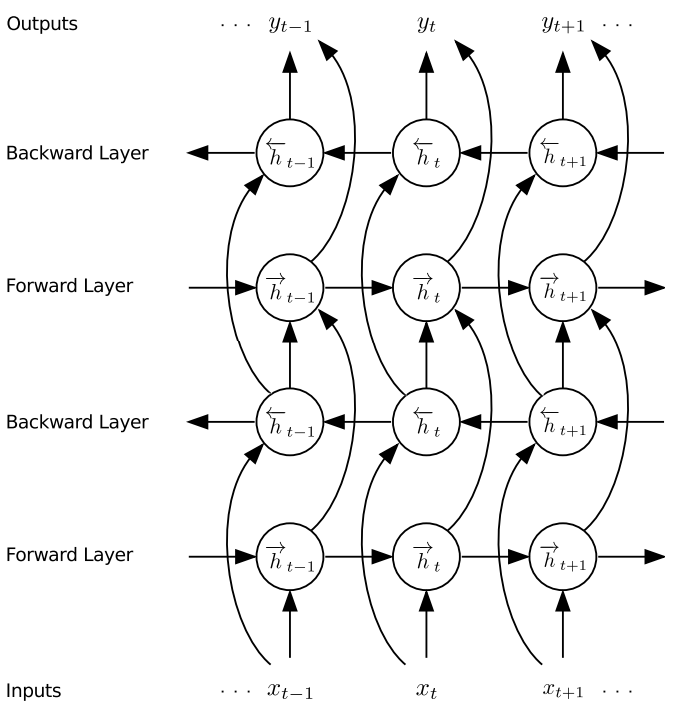
\includegraphics[height=.75\textheight,width=\textwidth,keepaspectratio]{images/arch_dbrnn}
        \caption{RNN bidirectionnel profond {\scriptsize\it -- Source : \cite{Graves13b}}}
    \end{figure}
    
\end{frame}

\begin{frame}{Architecture LSTM}
    
    \begin{figure}
        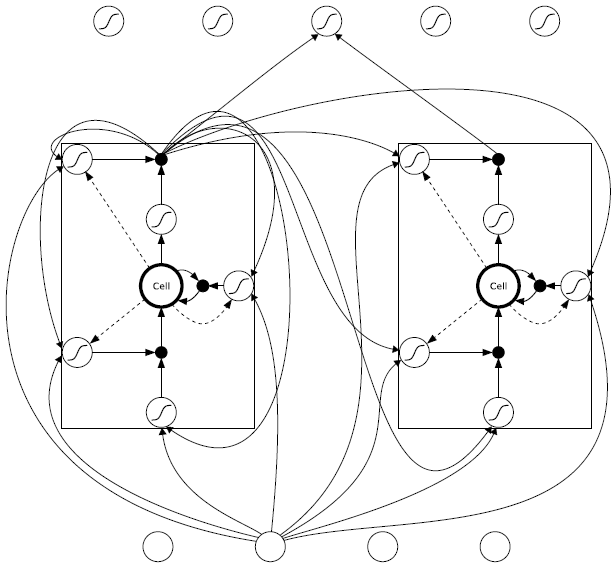
\includegraphics[height=.75\textheight,width=\textwidth,keepaspectratio]{images/arch_lstm}
        \caption{Architecture LSTM {\scriptsize\it -- Source : \cite{Graves12}}}
    \end{figure}
    
\end{frame}

\begin{frame}{LSTM bidirectionnel profond}
    
    \begin{figure}
        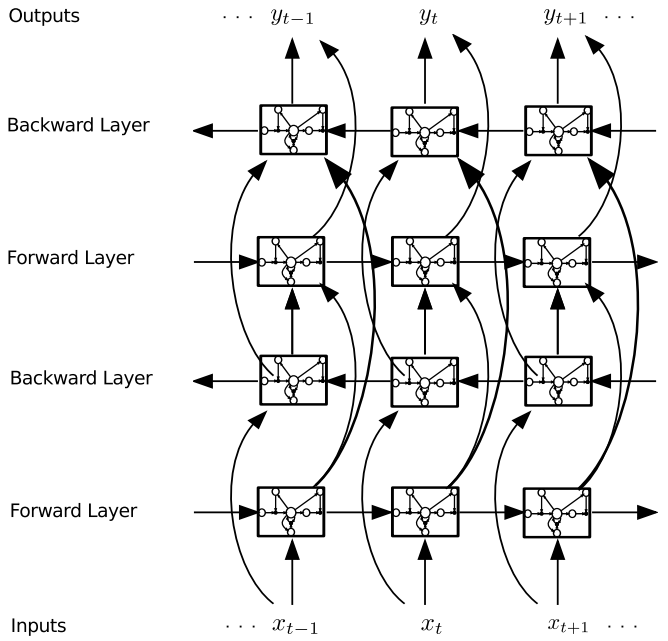
\includegraphics[height=.75\textheight,width=\textwidth,keepaspectratio]{images/arch_dblstm}
        \caption{LSTM bidirectionnel profond (DB-LSTM) {\scriptsize\it -- Source : \cite{Graves13b}}}
    \end{figure}
    
\end{frame}
